\documentclass[conference]{IEEEtran}

\usepackage{cite}
\usepackage{amsmath,amssymb}
\usepackage{graphicx}
\usepackage{booktabs}
\usepackage{multirow}
\usepackage{array}
\usepackage{url}
\usepackage{xcolor}
\usepackage{subcaption}
\usepackage{dblfloatfix}   % keep wide (figure*) floats in order; don't defer them to the end

\graphicspath{{figures/}}

% Relax float placement so figures are not all pushed to the end
\setcounter{topnumber}{3}
\setcounter{bottomnumber}{2}
\setcounter{totalnumber}{5}
\setcounter{dbltopnumber}{3}
\renewcommand{\topfraction}{0.95}
\renewcommand{\bottomfraction}{0.9}
\renewcommand{\textfraction}{0.05}
\renewcommand{\floatpagefraction}{0.8}
\renewcommand{\dbltopfraction}{0.95}
\renewcommand{\dblfloatpagefraction}{0.8}

\begin{document}

\title{Variance-Aware Synthetic Intent Generation for Network Slicing: A Controlled Comparison of Prompt-Level Diversity Techniques}

\author{
\IEEEauthorblockN{Author Name(s)}
\IEEEauthorblockA{
Department / Institution \\
Email: author@example.com}
}

\maketitle

\begin{abstract}
Intent-based management of 5G/6G networks maps natural-language operator requests to structured management actions, but training the underlying intent classifiers is limited by the scarcity of labeled, domain-specific telecom data. Large language models (LLMs) can synthesize such data at scale, yet the diversity and quality of the generated samples depend heavily on prompt design. This paper studies how prompt-level diversity strategies affect synthetic intent data for telecom network-slicing management. We propose a controlled framework that fixes the generation pipeline and varies only a modular variance-enhancement block, instantiating five literature-informed diversity strategies and a combined setting. Using a class-balanced synthetic dataset whose intent labels follow the network-slice management operations standardized by 3GPP, we assess each strategy along downstream learnability and both lexical and semantic diversity. The results reveal a consistent diversity--separability trade-off: combining all mechanisms produces the most diverse data, whereas scenario-grounded prompting produces the most learnable and semantically separable data. The framework provides a reproducible basis for selecting prompt-level diversity strategies when generating telecom intent data.
\end{abstract}

\begin{IEEEkeywords}
Intent-based networking, network slicing, large language models, synthetic data generation, prompt engineering, data diversity, intent classification.
\end{IEEEkeywords}

\section{Introduction}
\label{sec:intro}
AI-native network management is emerging as a key paradigm for automating 5G/6G network operations. Recent advances in large language models (LLMs) have enabled a wide range of network management tasks, including intent understanding, configuration assistance, orchestration, and troubleshooting \cite{bariahLLM}. Among these applications, Intent-Based Networking (IBN) enables operators to specify network objectives in natural language, which are subsequently translated into executable management actions \cite{mekracheIBN}. As a result, accurate intent understanding has become an essential component of AI-driven network automation.

Intent understanding is commonly formulated as an intent classification task, where natural-language requests are mapped to predefined operational actions. Training such models requires sufficiently large labeled datasets, yet domain-specific telecom data is scarce and costly to obtain due to expert annotation requirements. LLMs provide an alternative by generating synthetic training data, reducing reliance on manual labeling. The characteristics of synthetic data are strongly influenced by prompt design, affecting the diversity, coverage, and consistency of the generated samples \cite{nadasSynthetic}. These characteristics are expected to influence the effectiveness of downstream intent classification models. Despite recent advances in prompt engineering, its impact on synthetic dataset generation for telecom intent classification remains underexplored.

To address this gap, this paper proposes a controlled framework for evaluating prompt-level diversity strategies for synthetic dataset generation in telecom intent classification. The framework isolates the effect of prompt design by keeping the generation pipeline fixed while varying only the variance enhancement strategy. To evaluate the proposed framework in a realistic telecom setting, we construct a synthetic intent classification dataset based on network slicing management operations. The intent labels are derived from representative network slice management operations defined in the 3GPP management specifications, covering eight management actions related to slice lifecycle management, resource configuration, and slice information retrieval \cite{3gpp28531}. Grounding the label space in these standardized management operations keeps the generated data aligned with 3GPP-defined management interfaces and directly relevant to standards-based intent-driven slice management, rather than tied to an ad-hoc action set.

Our contributions are:
\begin{itemize}
    \item A controlled, reproducible synthetic-data generation \emph{framework} for network-slicing intent classification that varies only a single prompt-level diversity block over a fixed base prompt.
    \item Five literature-informed variance enhancement strategies (plus a combined setting), each mapped to its source work, adapted to the telecom intent-to-action task.
    \item A multi-axis evaluation---downstream learnability, lexical diversity, and embedding-based semantic diversity/separation---over a class-balanced set of $10{,}032$ generated examples, quantifying a diversity--separability trade-off and ranking the strategies with a transparent axis-weighted composite.
\end{itemize}

To support reproducibility, all code, prompts, and the generated dataset are publicly available.\footnote{\url{https://github.com/thedaffodil/variance-aware-intent-slicing}}

\section{Related Work}
\label{sec:related}

LLMs are widely used to synthesize training data when labeled examples are scarce or domain-specific, but recent work stresses that generated data must be judged on quality and diversity, not size alone. Studies on LLM text augmentation show that paraphrase-style generation can rival crowdsourcing in diversity and robustness~\cite{cegin2023chatgpt,dai2023auggpt}, while quality- and diversity-oriented synthesis must be balanced because the two objectives can pull in different directions~\cite{bao2025qualitydiversity}. These observations motivate evaluating our generated telecom intents along multiple complementary axes rather than by example count.

A recurring failure mode of LLM generation is template bias: even when asked to be diverse, models repeat openings, keywords, and scenarios. Cegin et al.~\cite{cegin2024diversity} compare explicit diversity incentives---taboo words, hints, and chaining---and find that taboo-word constraints raise lexical diversity while hint-based prompting can help downstream performance. Saparina and Lapata~\cite{saparina2024nlvariation} show that increasing natural-language variation improves generalization in semantic parsing, and DoAug~\cite{wang2025doaug} argues that the \emph{distribution} of generated samples, not just their number, should be diversified. Task-oriented dialogue research contributes structured recipes: SynTOD~\cite{samarinas2024syntod} drives generation from state-transition graphs, Finch and Choi~\cite{finch2024diversedst} show broad domain/slot coverage improves zero-shot dialogue state tracking, SyncTOD~\cite{saley2024synctod} uses task-specific hints, and schema-guided~\cite{kulkarni2024synthdst} and constrained~\cite{shin2021constrained} generation preserve the target schema. Benayas et al.~\cite{benayas2024intent} show LLM-generated labeled data improves intent-classifier training. Table~\ref{tab:sources} maps each of these to the variance enhancement strategy it inspires in our framework.

\begin{table}[t]
\centering
\small
\caption{Source work for each variance enhancement strategy.}
\label{tab:sources}
\begin{tabular}{p{0.22\linewidth} p{0.52\linewidth} l}
\toprule
\textbf{Strategy} & \textbf{Inspiration} & \textbf{Ref.} \\
\midrule
Taboo & Diversity incentives (taboo words) in LLM augmentation & \cite{cegin2024diversity} \\
NL+Dist & Natural-language variation; distribution-oriented augmentation & \cite{saparina2024nlvariation,wang2025doaug} \\
Scenario & State-graph TOD generation; diverse domain/slot coverage & \cite{samarinas2024syntod,finch2024diversedst} \\
Hints & Task-specific hints for TOD alignment & \cite{saley2024synctod} \\
Intent-Util & LLM-generated labeled data for intent classifiers & \cite{benayas2024intent} \\
ALL & Combine quality- and diversity-oriented synthesis & \cite{bao2025qualitydiversity} \\
\bottomrule
\end{tabular}
\end{table}

LLMs are increasingly applied to slice assignment, intent translation, and SDN automation. Hybrid neuro-symbolic methods combine LLM semantic grouping with optimization for constrained slice assignment~\cite{slice2025constrained}; end-to-end frameworks translate intents into policies and validate them through closed loops~\cite{e2e2025intent,hossain2025netintent}; and earlier IBN slicing systems map SLAs to slice configurations~\cite{ibnslicing2020}. Domain resources and dedicated slicing for LLM traffic have also appeared~\cite{tspecllm2025,llmslice2024}. Most of this work targets orchestration, execution, or agent behavior; comparatively little attention is paid to the \emph{quality of the synthetic intent data} used to build and test such systems. We address this data-generation and evaluation layer.

\section{Synthetic Intent Data Generation Framework}
\label{sec:datagen}

We propose a controlled framework in which a fixed base prompt defines the task and only a modular variance enhancement block changes across settings, so that differences in the generated data are attributable to the diversity mechanism rather than to the schema, examples, or formatting.

\subsection{Task and schema}
Each generated instance is a pair $\{\texttt{intent}, \texttt{slicing\_operation}\}$, where \texttt{intent} is a natural-language operator request, command, question, note, or incident message, and \texttt{slicing\_operation} is the single best-matching label. The label space is grounded in the network-slice provisioning and management operations standardized by 3GPP for the lifecycle and configuration of Network Slice Instances (NSIs)~\cite{3gpp28531}, so that the generated intents map onto standardized management actions rather than an ad-hoc taxonomy. It comprises eight labels spanning three operation families: (i) \emph{lifecycle}---\texttt{slice\_allocation} (create/assign an NSI) and \texttt{slice\_deallocation} (terminate and release); (ii) \emph{resource and quota configuration}---\texttt{slice\_rb\_update} (RAN resource-block ratio), \texttt{slice\_ue\_quota\_update} (max UEs), \texttt{slice\_pdu\_session\_quota\_update} (max concurrent PDU sessions), and \texttt{slice\_rrc\_con\_update} (max RRC connected users); and (iii) \emph{information retrieval}---\texttt{slice\_list} (list NSIs); plus \texttt{other} for in-domain but out-of-scope requests (e.g., alarm investigation, KPI monitoring, coverage or latency complaints).

\subsection{Base prompt}
A single fixed base prompt defines the model role (telecom slicing assistant), the task, the schema and label definitions, sixteen few-shot examples spanning command, operational-need, incident, monitoring, NOC-style, and out-of-scope phrasings, a six-step reasoning structure, the data-generation requirements (50 new examples, all labels used, no near-duplicates, exactly one correct label), and a JSON-only output format. A single placeholder, \texttt{[VARIANCE ENHANCEMENT BLOCK HERE]}, marks where the variance block is injected.

\subsection{Variance enhancement strategies}
We instantiate five single strategies and one combined setting; Table~\ref{tab:settings} describes the block injected in each (the source works were given in Table~\ref{tab:sources}). Each block is inserted alone into the same base prompt, and the model is asked to generate 50 new examples using all eight labels and avoiding near-duplicates.

\begin{table}[t]
\centering
\small
\caption{Variance enhancement strategies (one block injected per setting).}
\label{tab:settings}
\begin{tabular}{p{0.20\linewidth} p{0.71\linewidth}}
\toprule
\textbf{Strategy} & \textbf{What the block instructs} \\
\midrule
Taboo & Forbid repetitive command openings (Create, Update, Set, Increase, List, Delete, Show, Remove); encourage context-first phrasings (incidents, congestion, capacity warnings). \\
\addlinespace
NL+Dist & Produce realistic operator language (NOC notes, incidents, monitoring, shorthand) and balance across labels, scenarios, sentence length, identifiers, numeric patterns, and styles. \\
\addlinespace
Scenario & Start from a realistic telecom situation (event congestion, IoT growth, emergency response, mining telemetry, $\dots$) rather than the operation name; enforce broad domain coverage. \\
\addlinespace
Hints & Give explicit task hints: operation selection by goal, grounding to stated values, realism, and schema consistency. \\
\addlinespace
Intent-Util & Ask for semantically clear but linguistically diverse, non-keyword-driven intents (e.g., not every \texttt{slice\_rb\_update} contains ``RB allocation''). \\
\addlinespace
ALL & Apply all five blocks in a single prompt. \\
\bottomrule
\end{tabular}
\end{table}

\subsection{Generation pipeline}
Generation is automated by a task runner. A task file lists, per setting, a task identifier and the enhancement block(s) to inject. For each run the runner reads the fixed base prompt, injects the block(s), calls the LLM through its CLI over \emph{stdin} (the assembled prompt exceeds 15{,}000 characters, beyond the Windows command-line limit), and stores the raw JSON output; the exact prompt used is also saved for auditability. Runs execute concurrently via a thread pool with a filename lock that reserves each output slot atomically.

\subsection{Generated corpus}
For each of the six settings we generate a class-balanced set of $1{,}672$ intents with a uniform distribution over the eight labels ($209$ per label), giving a corpus of $10{,}032$ examples. All generated files pass JSON/schema validation with \emph{zero} invalid labels, and the uniform label distribution (normalized label entropy $=1.0$) rules out class imbalance as a confound in the comparison across settings.

\section{Evaluation Framework}
\label{sec:eval}

We evaluate each setting on two axes: \emph{separability} (how learnable/separable the data is) and \emph{diversity} (how varied the intents are). Ground-truth label correctness is not available, so we report schema validity together with downstream learnability and semantic separation as complementary proxies for quality. Table~\ref{tab:metrics} summarizes the metrics.

\emph{Notation.} Let $D=\{(x_i,y_i)\}_{i=1}^{N}$ be a setting's generated examples, where $x_i$ is the intent, $y_i\in\mathcal{L}$ its label ($|\mathcal{L}|=8$), and $e_i$ the L2-normalized sentence embedding of $x_i$, so that $\cos(e_i,e_j)=e_i^{\top}e_j$.

\begin{table}[t]
\centering
\small
\caption{Evaluation metrics (Dir.: $\uparrow$ higher is better, $\downarrow$ lower is better).}
\label{tab:metrics}
\begin{tabular}{llcl}
\toprule
\textbf{Metric} & \textbf{Axis} & \textbf{Dir.} & \textbf{What it measures} \\
\midrule
Accuracy / Macro-F1 & Separability & $\uparrow$ & learnability (5-fold CV) \\
Sep.\ gap & Separability & $\uparrow$ & semantic class distinctness \\
MATTR & Diversity & $\uparrow$ & vocabulary richness \\
Distinct-2 & Diversity & $\uparrow$ & bigram variety \\
Self-BLEU & Diversity & $\downarrow$ & inter-sentence repetition \\
Sem-Div & Diversity & $\uparrow$ & embedding-space spread \\
Dispersion & Diversity & $\uparrow$ & spread around centroid \\
\bottomrule
\end{tabular}
\end{table}

\subsection{Separability}
\emph{Downstream learnability} trains a TF--IDF ($1$--$2$ grams, max $5000$ features) + logistic-regression classifier under stratified $5$-fold \texttt{cross\_val\_predict}, so each example is predicted once ($\hat{y}_i$) while held out. We report accuracy and macro-F1:
\begin{equation}
\mathrm{Acc}=\frac{1}{N}\sum_{i=1}^{N}\mathbf{1}(\hat{y}_i=y_i),
\end{equation}
where higher values mean the intent text strongly signals its label (separability, not ground-truth correctness). \emph{Semantic separation} is the class separation gap
\begin{equation}
\Delta_{\mathrm{sep}}=\overline{\cos}_{\,y_i=y_j}-\overline{\cos}_{\,y_i\neq y_j},
\end{equation}
the within-class minus between-class mean cosine similarity; higher means classes are more distinct.

\subsection{Diversity}
\emph{Lexical} diversity uses MATTR (moving-average type-token ratio, window $50$) for length-robust vocabulary richness, Distinct-$n$, and Self-BLEU:
\begin{equation}
\text{Distinct-}n=\frac{|\{\text{unique }n\text{-grams}\}|}{|\{\text{all }n\text{-grams}\}|},
\end{equation}
\begin{equation}
\text{Self-BLEU}=\frac{1}{N}\sum_{i=1}^{N}\text{BLEU}\big(x_i,\{x_j\}_{j\neq i}\big),
\end{equation}
where higher Distinct-$n$ and \emph{lower} Self-BLEU indicate more diverse text. \emph{Semantic} diversity uses the embeddings:
\begin{equation}
\text{Sem-Div}=1-\frac{2}{N(N-1)}\sum_{i<j}\cos(e_i,e_j),
\end{equation}
together with centroid dispersion (mean $1-\cos$ to the setting centroid); higher means a wider spread in semantic space. All metrics are computed per setting with a fixed random seed for reproducibility. Semantic metrics use \texttt{all-mpnet-base-v2} embeddings ($768$-dimensional, L2-normalized); the two-dimensional map uses PCA(50) followed by t-SNE.

\subsection{Composite ``goodness'' and its weighting}
To summarize, we combine the axes into a single score. Let $\hat{\cdot}$ denote min--max normalization of a metric across the six settings, oriented so that higher is better ($\hat{b}$ uses $1-\text{Self-BLEU}$). We define a separability score $S$ and a diversity score $V$ from four sub-scores:
\begin{align}
L &= \tfrac{1}{2}(\hat{a}+\hat{f}), & P &= \hat{g}, \\
X &= \tfrac{1}{3}(\hat{m}+\hat{d}+\hat{b}), & Y &= \tfrac{1}{2}(\hat{s}+\hat{p}),
\end{align}
where $\hat{a},\hat{f},\hat{g}$ are normalized accuracy, macro-F1, and separation gap, and $\hat{m},\hat{d},\hat{b},\hat{s},\hat{p}$ are normalized MATTR, Distinct-2, $1-$Self-BLEU, Sem-Div, and dispersion. The axis and overall scores are
\begin{equation}
S=\tfrac{1}{2}(L+P),\quad V=\tfrac{1}{2}(X+Y),\quad G=\tfrac{1}{2}(S+V).
\end{equation}
We weight the two \emph{axes} $S$ and $V$ equally rather than averaging raw metrics, because a flat per-metric mean would silently over-weight whichever axis has more metrics; accuracy and macro-F1 are grouped in $L$ because they are near-redundant. This is a transparent default, not a tuned weighting.

\section{Results}
\label{sec:results}

\subsection{Learnability and diversity}
Table~\ref{tab:main} reports the per-setting metrics on the balanced set. All settings are highly separable ($\geq 0.975$ accuracy), confirming the generated intents carry a learnable label signal; scenario-path and natural-language prompting are the most separable ($0.988$) and also achieve the largest semantic class separation, while intent-classification-utility is the least separable ($0.975$)---consistent with its deliberately non-keyword intents. On diversity, ALL dominates the lexical axis by a clear margin (Self-BLEU $0.299$ vs.\ $0.329$--$0.386$; highest Distinct-2 and MATTR). Semantic diversity is led by Intent-Util and ALL, which occupy the widest embedding-space spread.

\begin{table*}[t]
\centering
\small
\caption{Per-setting results on the balanced set. Arrows give the better direction; best per column in bold. Learnability is 5-fold CV; semantic metrics use \texttt{all-mpnet-base-v2}.}
\label{tab:main}
\begin{tabular}{l ccc cccc}
\toprule
 & \multicolumn{3}{c}{\textbf{Separability}} & \multicolumn{4}{c}{\textbf{Diversity}} \\
\cmidrule(lr){2-4}\cmidrule(lr){5-8}
\textbf{Setting} & Acc$\uparrow$ & M-F1$\uparrow$ & Sep.\ gap$\uparrow$ & MATTR$\uparrow$ & Dist-2$\uparrow$ & Self-BLEU$\downarrow$ & Sem-Div$\uparrow$ \\
\midrule
Taboo        & 0.981 & 0.981 & 0.167 & 0.844 & 0.399 & 0.329 & 0.716 \\
NL+Dist      & \textbf{0.988} & \textbf{0.988} & 0.173 & 0.843 & 0.410 & 0.345 & 0.700 \\
Scenario     & \textbf{0.988} & \textbf{0.988} & \textbf{0.183} & 0.848 & 0.386 & 0.367 & 0.697 \\
Hints        & 0.986 & 0.986 & 0.173 & 0.837 & 0.390 & 0.368 & 0.706 \\
Intent-Util  & 0.975 & 0.975 & 0.158 & 0.835 & 0.368 & 0.386 & \textbf{0.722} \\
ALL          & 0.978 & 0.978 & 0.167 & \textbf{0.860} & \textbf{0.431} & \textbf{0.299} & 0.721 \\
\bottomrule
\end{tabular}
\end{table*}

\subsection{Semantic map and coverage}
Fig.~\ref{fig:tsne} projects the balanced embeddings to two dimensions (PCA(50)$\rightarrow$t-SNE) for three settings chosen to span the corners of the trade-off space: Scenario (most separable), ALL (most lexically diverse), and Intent-Util (highest semantic diversity but lowest class separation). In every panel the eight operations form visibly distinct clusters, and each setting populates \emph{all} clusters. Two observations follow. First, the clear cluster structure explains the uniformly high learnability in Table~\ref{tab:main}: even the least separable setting still yields well-formed clusters. Second, because no setting collapses onto a sub-region or omits a class, the strategies differ in \emph{how tightly} they fill the space rather than in \emph{which} regions they cover---Scenario's clusters are the most compact and best separated, whereas Intent-Util's are more diffuse and overlapping, matching its lower separation gap.

\begin{figure*}[t]
\centering
\begin{subfigure}[t]{0.32\textwidth}
\centering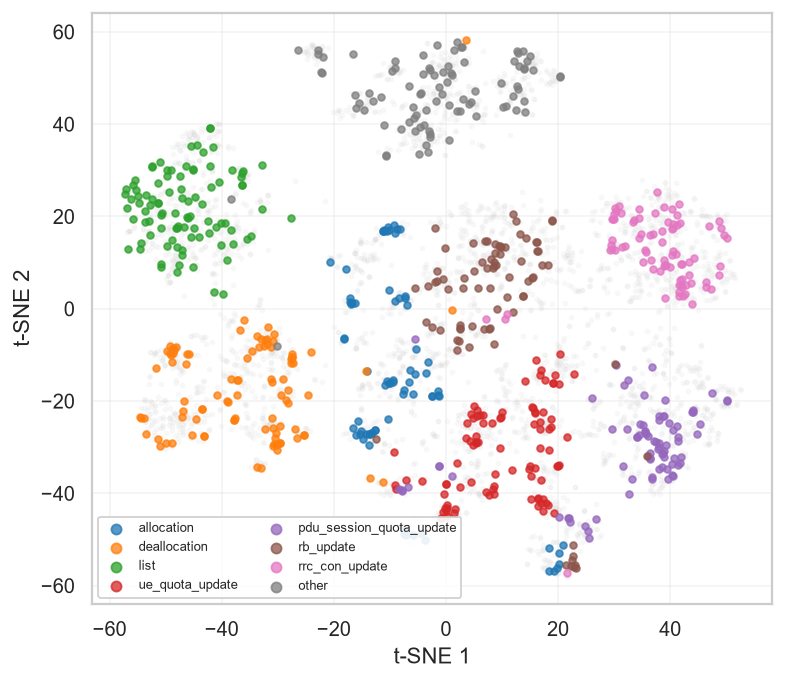
\includegraphics[width=\linewidth]{fig_tsne_a.png}
\caption{Scenario --- most separable / compact clusters.}
\label{fig:tsne_a}
\end{subfigure}\hfill
\begin{subfigure}[t]{0.32\textwidth}
\centering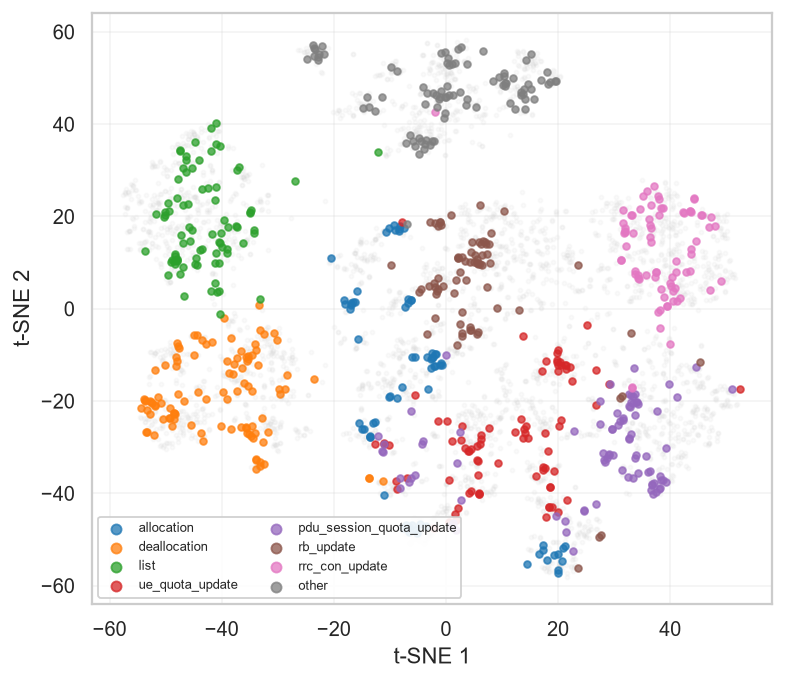
\includegraphics[width=\linewidth]{fig_tsne_b.png}
\caption{ALL --- most lexically diverse.}
\label{fig:tsne_b}
\end{subfigure}\hfill
\begin{subfigure}[t]{0.32\textwidth}
\centering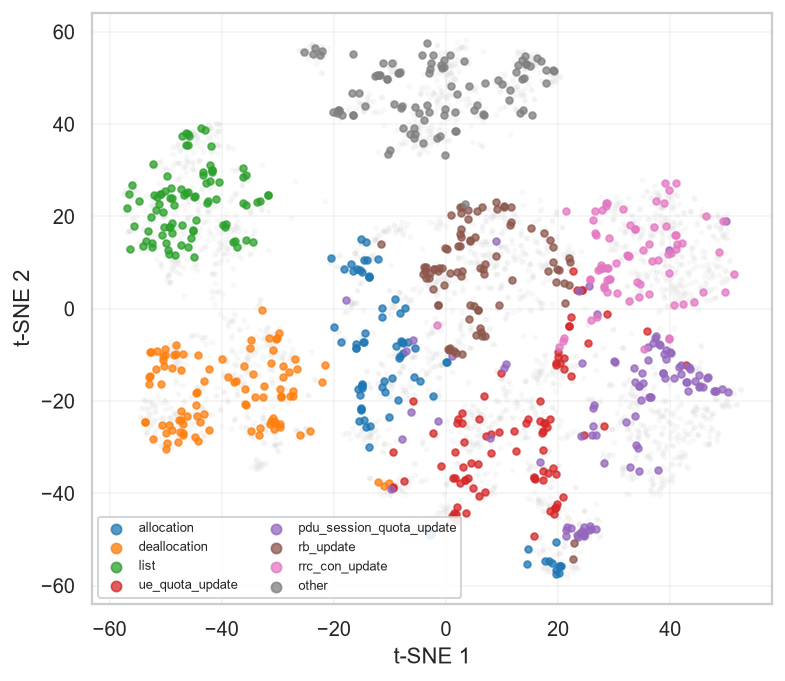
\includegraphics[width=\linewidth]{fig_tsne_c.png}
\caption{Intent-Util --- highest semantic diversity, most overlap.}
\label{fig:tsne_c}
\end{subfigure}
\caption{Shared t-SNE projection of the balanced embeddings. Each panel colors one setting's examples by slicing operation with the other settings greyed; coordinates are common across panels. The eight operations form distinct clusters and every setting covers all of them.}
\label{fig:tsne}
\end{figure*}

\subsection{The diversity--separability trade-off}
Fig.~\ref{fig:tradeoff} plots lexical diversity ($1-$Self-BLEU) against separability. A broad trade-off is visible: the most lexically diverse setting (ALL) sits at the high-diversity, mid-separability corner, while the most separable settings (Scenario, NL+Dist) are markedly less lexically diverse. Intent-Util is the informative exception---lowest on both lexical diversity and separability, yet highest on \emph{semantic} diversity (Table~\ref{tab:main})---which shows that lexical and semantic diversity are not interchangeable: its non-keyword intents reuse surface patterns (lower Distinct-2/higher Self-BLEU) while spreading widely in meaning. In practice this means a single diversity number is misleading; a technique must be placed on both the lexical and the semantic axis before judging it.

\begin{figure}[!t]
\centering
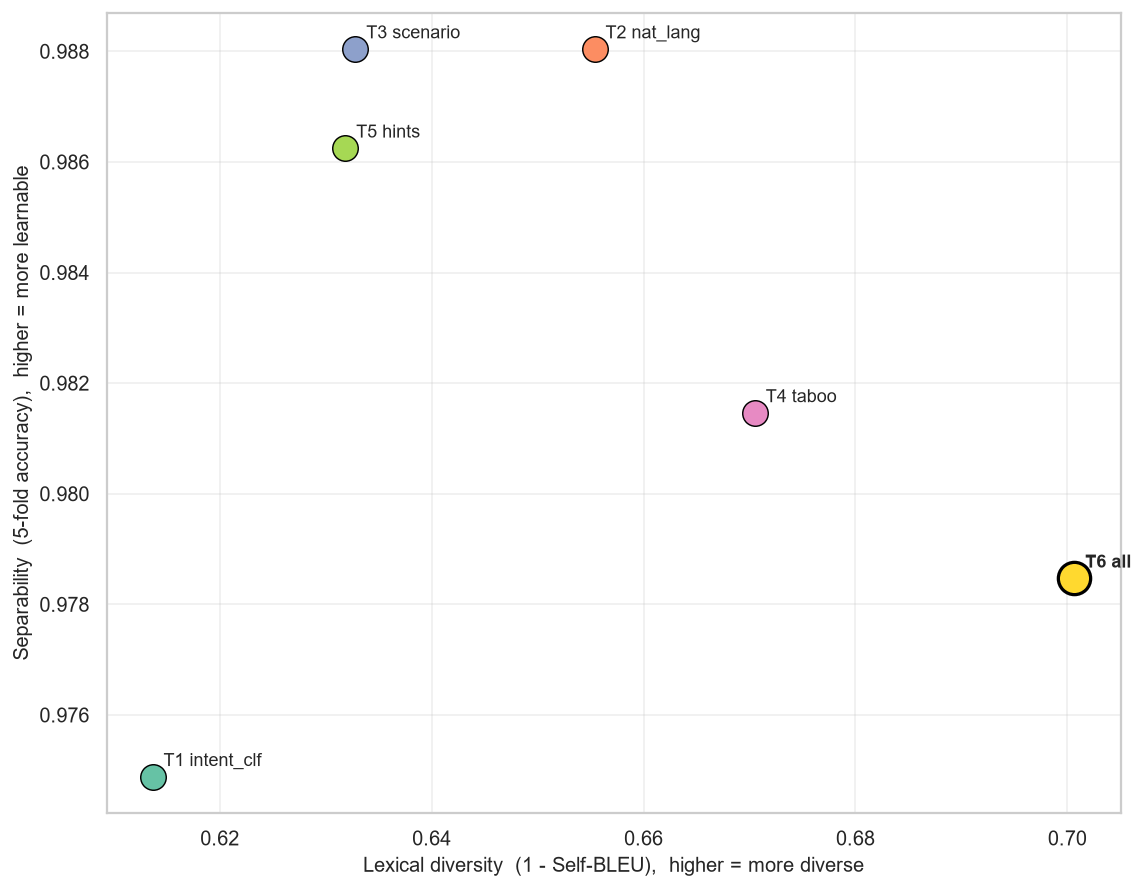
\includegraphics[width=\linewidth]{fig_tradeoff.png}
\caption{Lexical diversity ($1-$Self-BLEU) vs.\ separability (5-fold accuracy). ALL is the most lexically diverse; Scenario and NL+Dist are the most separable; Intent-Util is low on both lexical axes despite high semantic diversity.}
\label{fig:tradeoff}
\end{figure}

\subsection{Class-level semantic structure}
Fig.~\ref{fig:opsim} reports the mean pairwise cosine similarity between operation classes on the pooled balanced set. The diagonal (within-class cohesion) is highest for \texttt{slice\_list} and \texttt{slice\_rrc\_con\_update}, while the most confusable off-diagonal pairs are resource-block vs.\ RRC-connection updates and UE-quota vs.\ PDU-session-quota updates---operations that are genuinely close in intent and share vocabulary. The \texttt{other} class is the least cohesive, as expected for an open, out-of-scope category. This structure is stable across settings and identifies exactly which operations a downstream classifier is most likely to confuse, guiding targeted data collection.

\begin{figure}[!t]
\centering
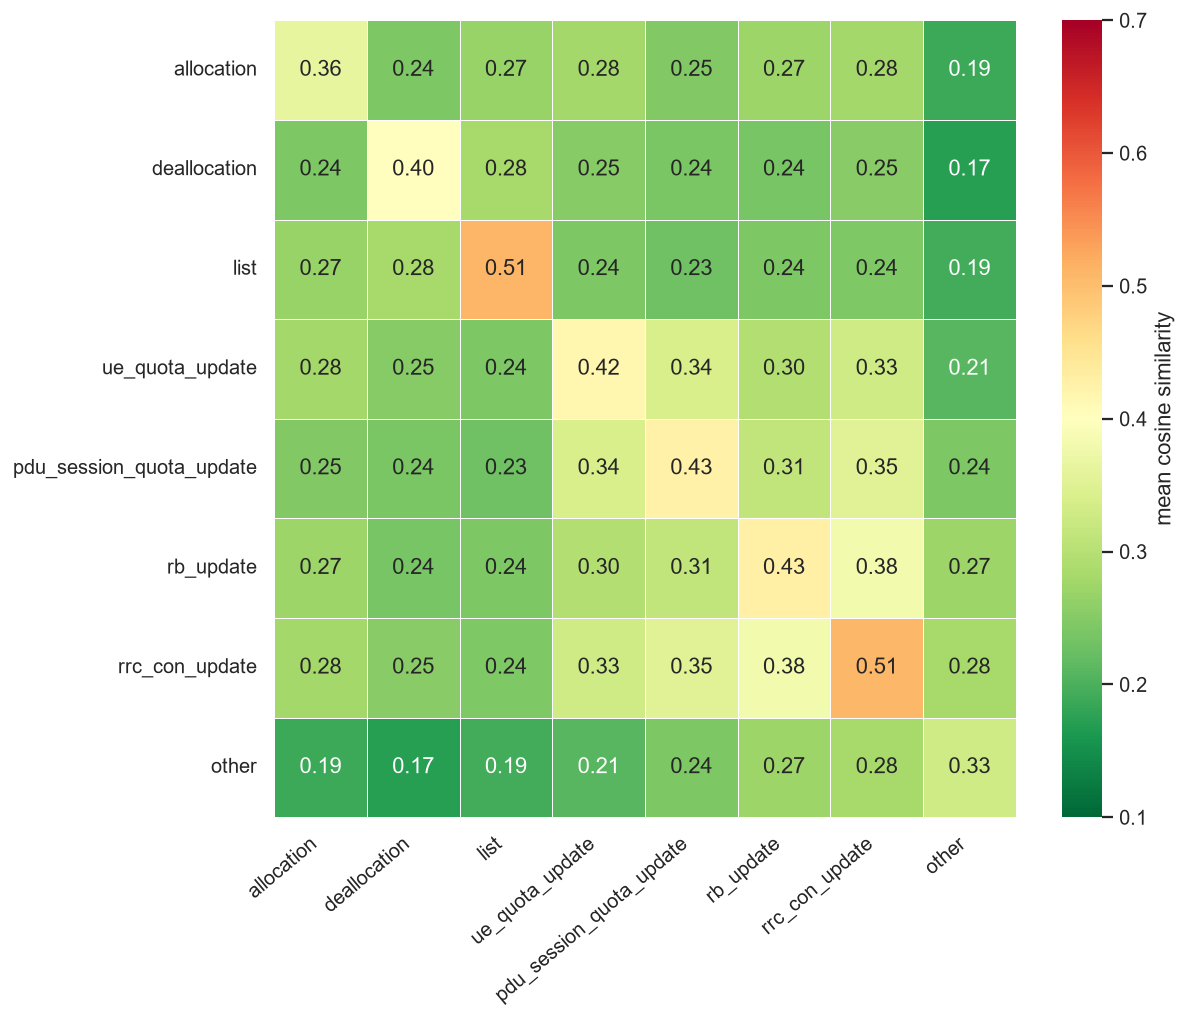
\includegraphics[width=\linewidth]{fig_op_similarity.png}
\caption{Mean cosine similarity between operation classes (pooled balanced set). Diagonal: within-class cohesion; off-diagonal: confusability.}
\label{fig:opsim}
\end{figure}

\subsection{Overall comparison and composite ranking}
Table~\ref{tab:goodness} reports the axis-weighted composite. The two axes expose two clean strategies: Scenario maximizes separability ($0.999$) but is weak on diversity, whereas ALL nearly maximizes diversity ($0.950$) and, under equal axis weights, ranks first overall ($G=0.627$), with Scenario a close second ($0.585$). Fig.~\ref{fig:heatmap} shows all metrics jointly after normalization: although it compactly encodes every criterion, its density makes it best read as a summary rather than a primary result---ALL is green across the diversity columns and weaker on separability, while Scenario shows the opposite profile, visually confirming the trade-off established above.

\begin{table}[t]
\centering
\small
\caption{Axis-weighted composite on the balanced set (normalized $0$--$1$, sorted).}
\label{tab:goodness}
\begin{tabular}{lccc}
\toprule
\textbf{Setting} & \textbf{Separability $S$} & \textbf{Diversity $V$} & \textbf{Goodness $G$} \\
\midrule
ALL          & 0.304 & \textbf{0.950} & \textbf{0.627} \\
Scenario     & \textbf{0.999} & 0.171 & 0.585 \\
NL+Dist      & 0.797 & 0.288 & 0.542 \\
Taboo        & 0.431 & 0.634 & 0.533 \\
Hints        & 0.733 & 0.288 & 0.510 \\
Intent-Util  & 0.000 & 0.500 & 0.250 \\
\bottomrule
\end{tabular}
\end{table}

\begin{figure*}[t]
\centering
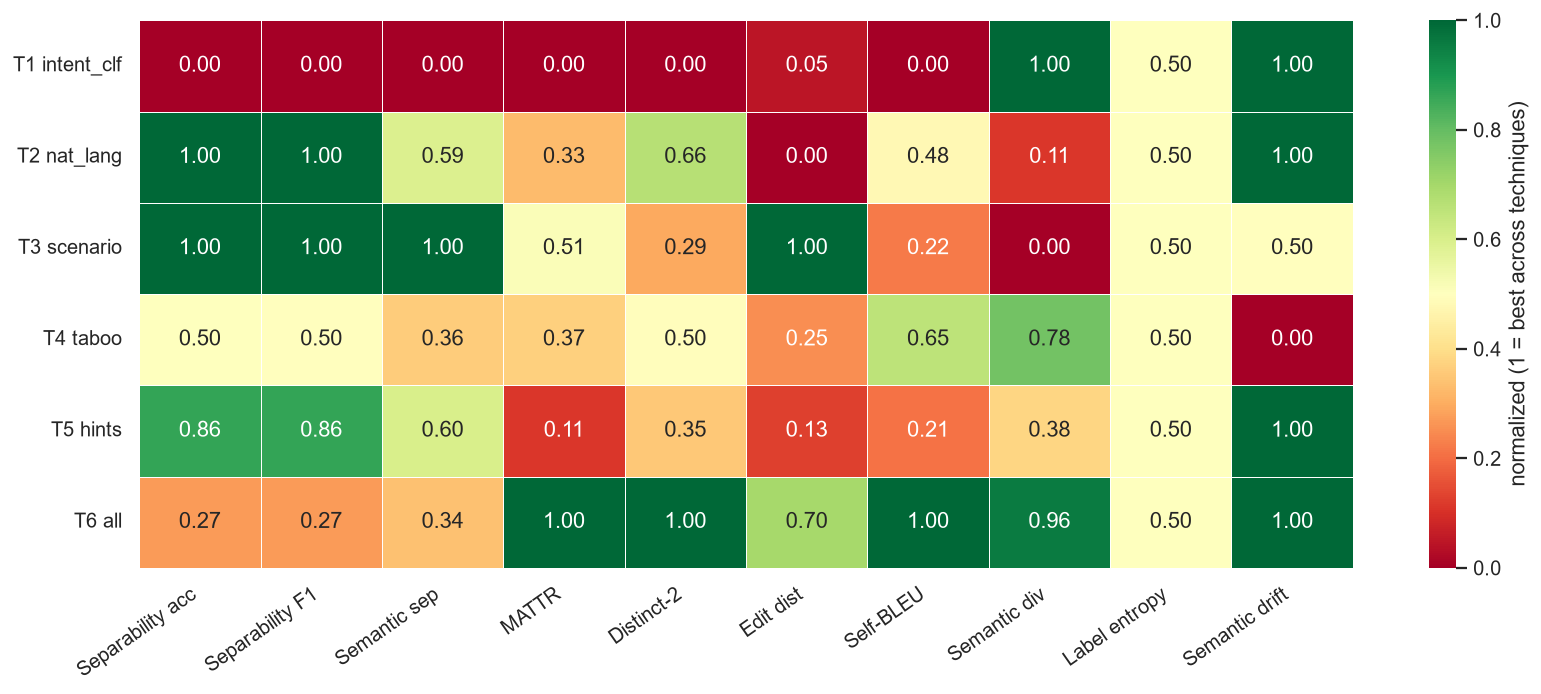
\includegraphics[width=0.95\textwidth]{fig_heatmap.png}
\caption{Normalized comparison across all metrics (each column min--max scaled, oriented so green is best). ALL is best on the diversity columns but weaker on separability; Scenario shows the opposite profile. The figure encodes every criterion at once and is included as a compact overview.}
\label{fig:heatmap}
\end{figure*}

\section{Discussion}
\label{sec:discussion}

On the balanced set the strategies separate into two regimes. Combining all mechanisms (ALL) maximizes lexical and semantic diversity and, because it is still highly learnable, ranks first under equal axis weights; it is the natural choice when coverage and novelty matter most. Scenario-path prompting is the opposite pole: grounding generation in concrete telecom situations yields the most separable and most semantically distinct classes at the cost of lexical variety, making it preferable when a clean, learnable classifier is the goal. Intent-classification-utility is a cautionary case: its non-keyword design maximizes semantic diversity but lowers both lexical diversity and separability, so ``diversity'' must be read on both axes. Because all settings preserve perfect schema validity and (by construction) balanced labels, the diversity mechanisms expand surface and scenario variety without destabilizing label structure. A practical recipe follows: use scenario/hint prompting when learnability is paramount, the combined setting when breadth is paramount, and blend the two to balance the trade-off; the class-similarity structure additionally flags the operation pairs most in need of disambiguating data.

\section{Threats to Validity}
\label{sec:threats}

First, we measure schema validity and proxies for quality (learnability, semantic separation) rather than ground-truth label correctness; an independent LLM judge or human verification would close this gap. Second, metrics are point estimates without confidence intervals, so small between-setting differences should be read cautiously. Third, embedding-based metrics depend on the encoder; we use a strong general-purpose model but a telecom-adapted encoder could refine absolute values. Finally, results may depend on the specific LLM, decoding settings, and prompt wording, and other diversity strategies may yield different trade-offs.

\section{Conclusion}
\label{sec:conclusion}

We presented a controlled framework for synthesizing network-slicing intent data and a study of prompt-level diversity strategies within it. Holding a base prompt fixed and varying only a modular variance block, we generated a class- and setting-balanced corpus of $10{,}032$ examples ($1{,}672$ per setting) and evaluated the strategies on learnability, lexical diversity, and embedding-based semantic diversity and separation. The strategies trace a clear diversity--separability trade-off: combining all mechanisms maximizes diversity and ranks first under equal weighting, scenario-path prompting maximizes separability, and lexical and semantic diversity are shown to be distinct axes. Because the label space is grounded in the 3GPP-standardized slice management operations, the framework produces synthetic data aligned with standardized network-management interfaces, supporting the development and benchmarking of standards-compliant intent-based slice management. By mapping each strategy to its literature source and releasing a transparent, reproducible evaluation, the framework offers practical guidance for designing generation prompts in telecom intent-based management. Future work will add LLM-judge label-correctness scoring, cross-run consistency, and statistical significance testing.

\bibliographystyle{IEEEtran}
\bibliography{references}

\end{document}
